\section{Monopole Antenna -- Version 1}
Pad too small. fr4 support. 

\begin{figure}[htbp]
   \begin{subfigure}[b]{0.49\linewidth}
        \centering
        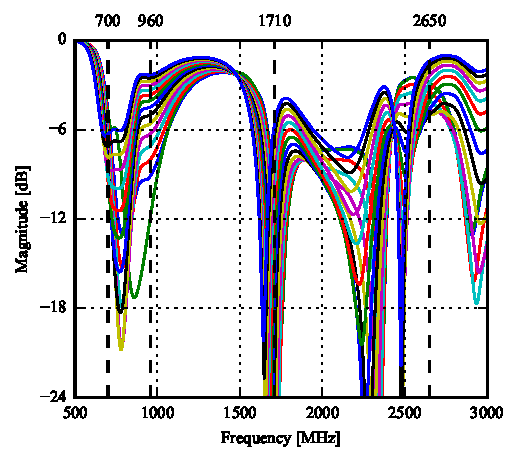
\includegraphics{img/tech_sol/monopole/prototype_v1/s11}
        \caption{$S_{11}$, sweeping $C_1$ and fixing $C_2$.}
        \label{fig:ant1_s11}
    \end{subfigure}
    \hfill
    \begin{subfigure}[b]{0.49\linewidth}
        \centering
        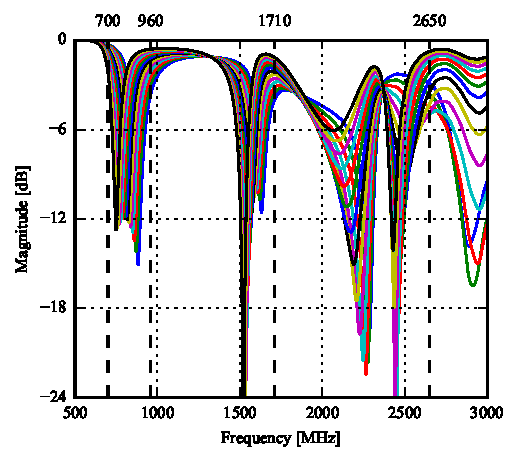
\includegraphics{img/tech_sol/monopole/prototype_v1/s22}
        \caption{$S_{22}$, sweeping $C_2$ and fixing $C_1$.}
        \label{fig:ant1_s22}
    \end{subfigure}
~
    \begin{subfigure}[b]{0.49\linewidth}
        \centering
        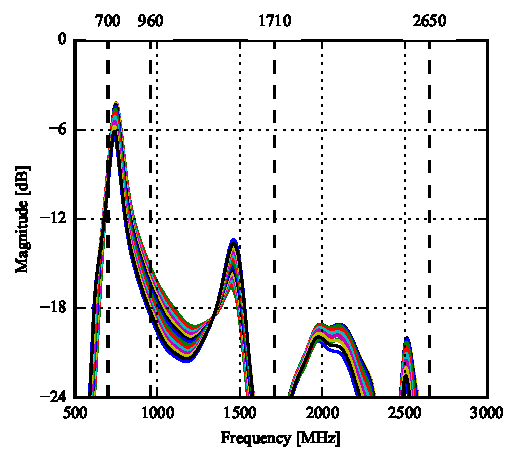
\includegraphics{img/tech_sol/monopole/prototype_v1/s21-s11}
        \caption{$S_{21}$, sweeping $C_1$ and fixing $C_2$.}
        \label{fig:ant1_s11}
    \end{subfigure}
    \hfill
    \begin{subfigure}[b]{0.49\linewidth}
        \centering
        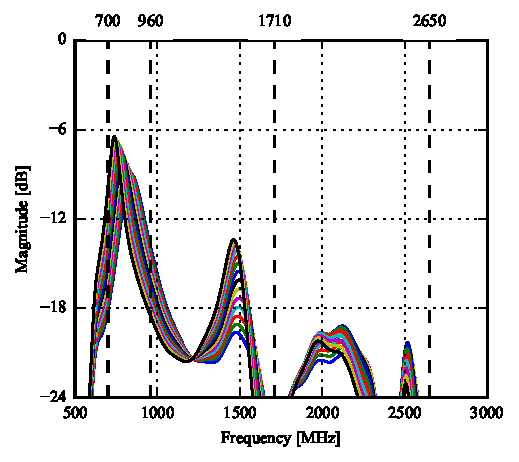
\includegraphics{img/tech_sol/monopole/prototype_v1/s21-s22}
        \caption{$S_{21}$, sweeping $C_2$ and fixing $C_1$.}
        \label{fig:ant1_s22}
    \end{subfigure}
    \caption{S-parameter sweep in free space for tuning the shunt capacitor of each antenna, $C_1$ and $C_2$ for port 1 and 2, respectively. Port 1 is the top antenna and port 2 is the side antenna.}
    \label{fig:sparam_mono_sim_proto}
\end{figure}

\begin{figure}
    \centering
    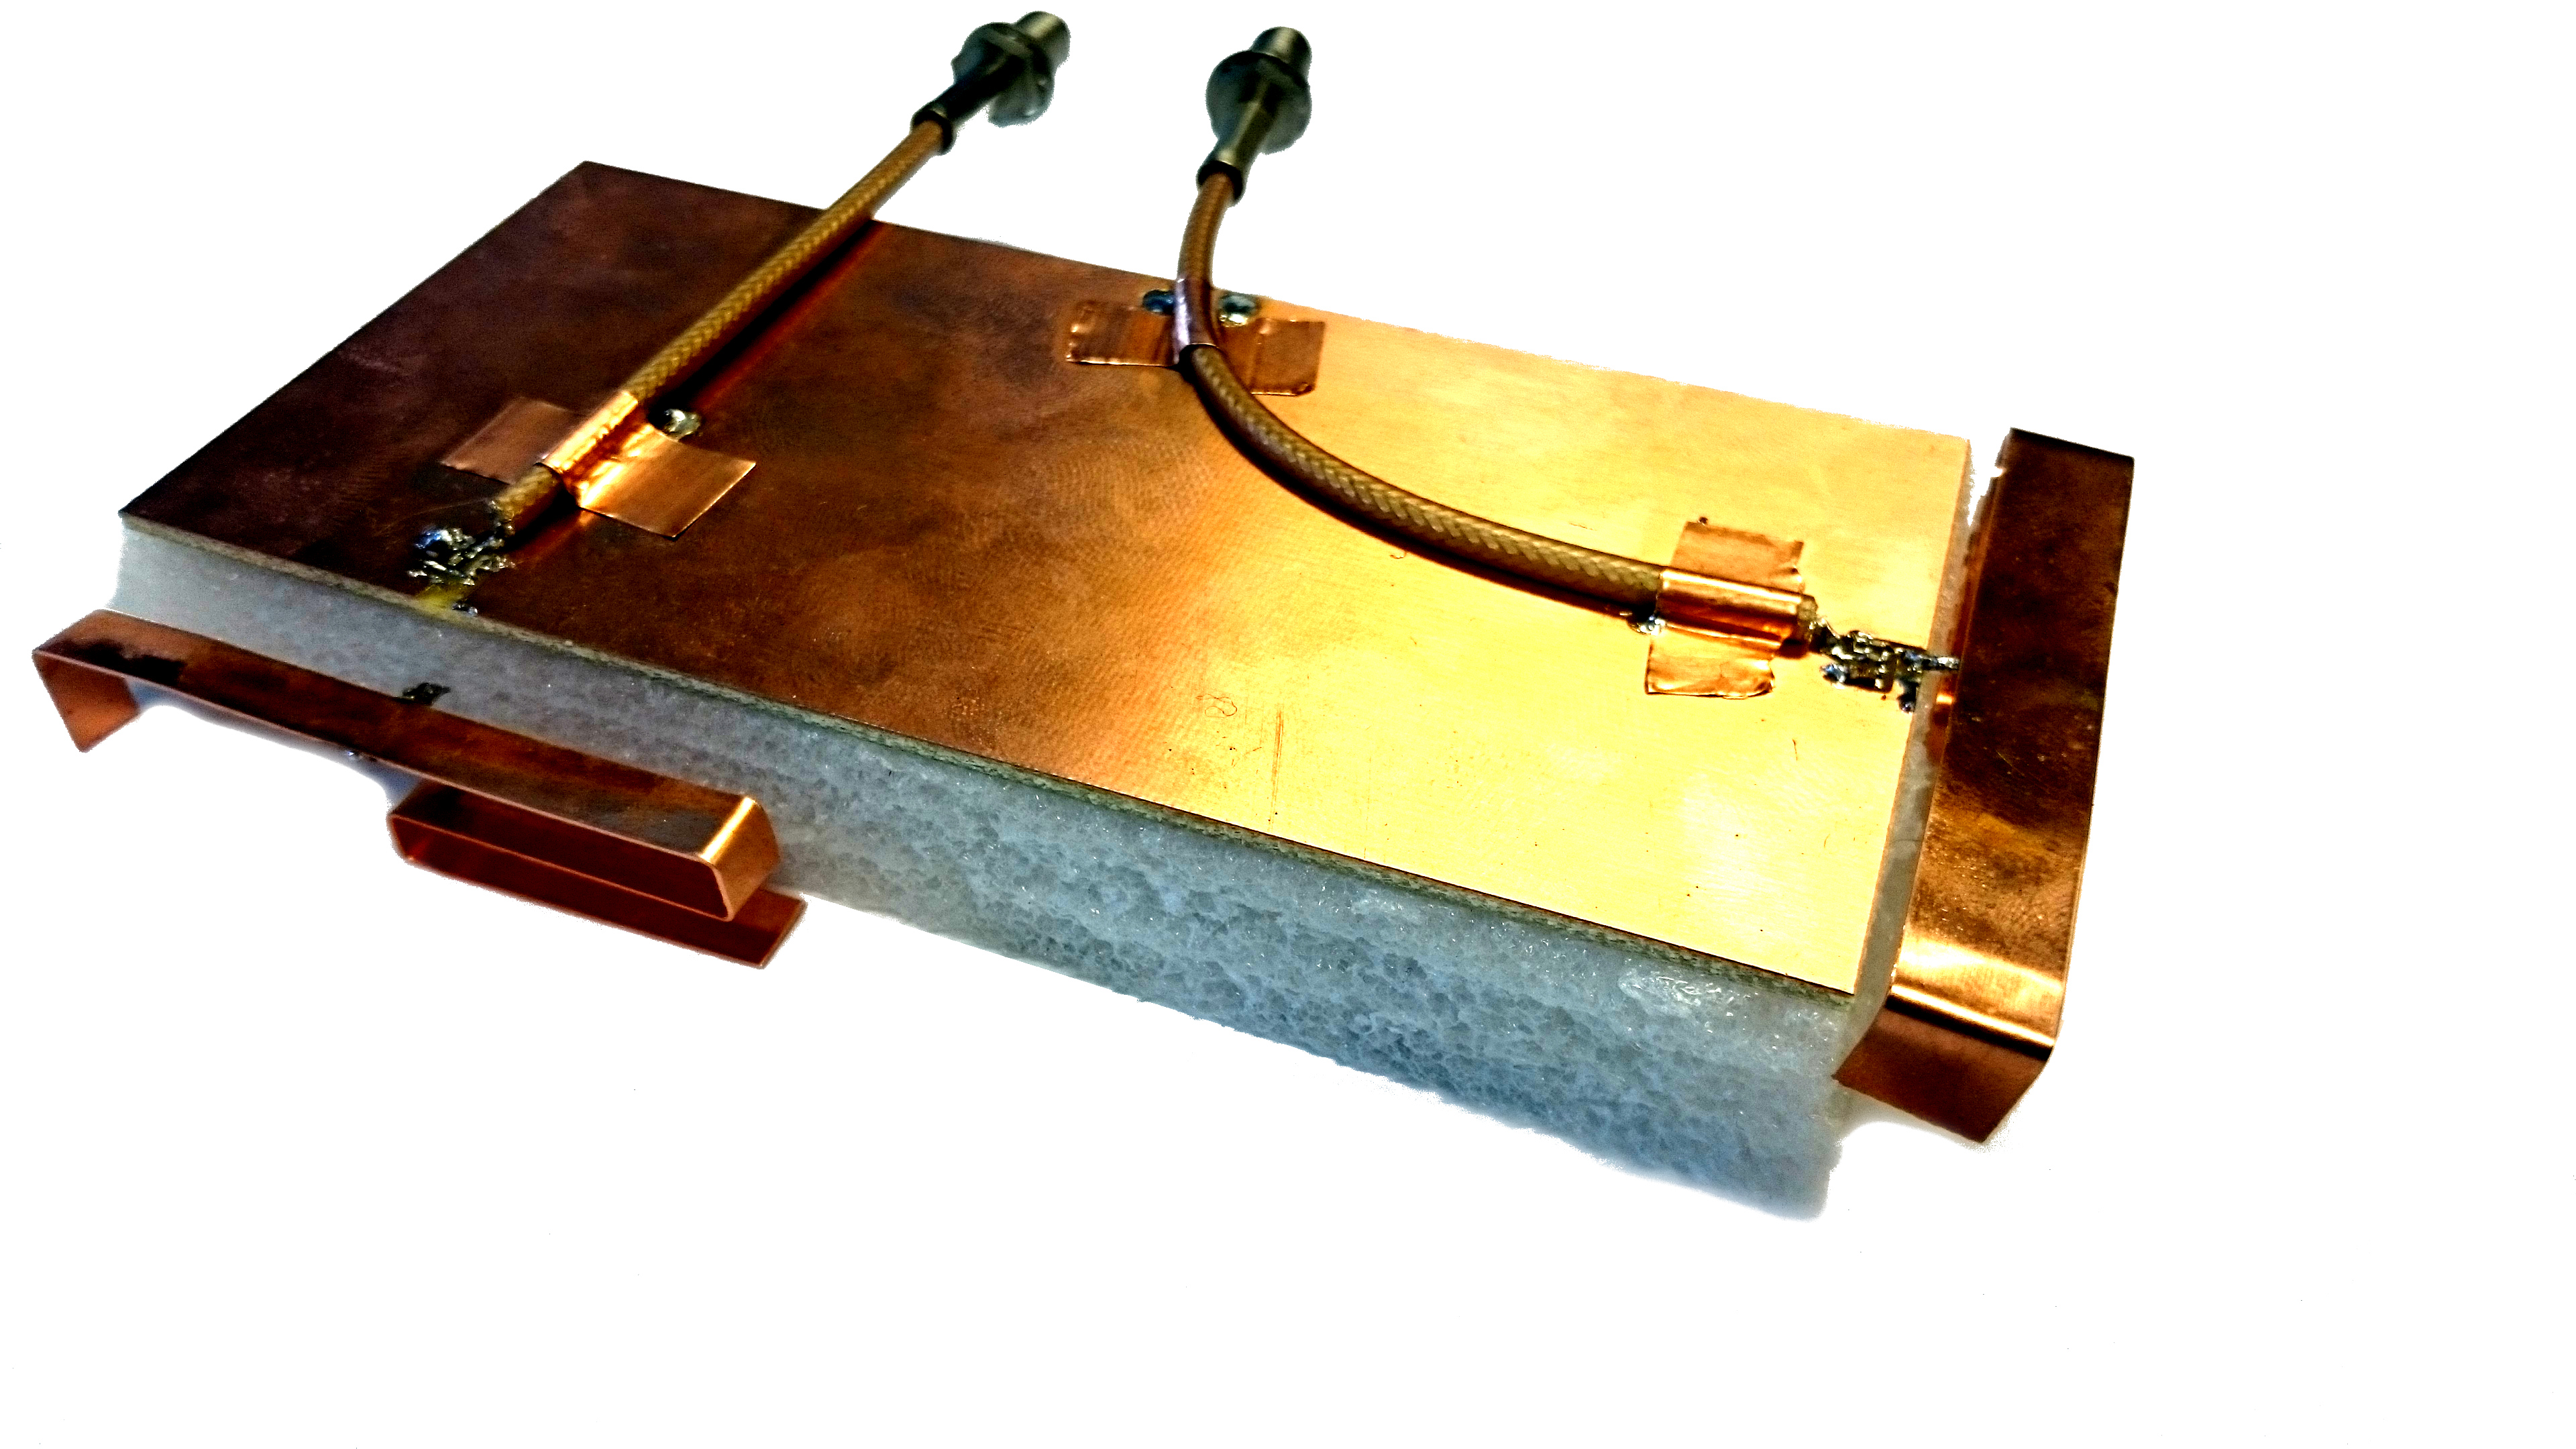
\includegraphics[scale=0.1]{img/tech_sol/monopole/prototype/monopole_v1}
    \caption{Monopole prototype version 1}
    \label{fig:ant1_proto1_3d}
\end{figure}
